\documentclass[11pt]{article}
\usepackage[margin=1in]{geometry}
\usepackage{times}
\usepackage{graphicx}
\usepackage{amsmath}
\usepackage{booktabs}
\usepackage{array}
\usepackage{tabularx}
\usepackage{cite}
\usepackage[hidelinks]{hyperref}
\usepackage{url}
\graphicspath{{figures/}}
\renewcommand{\arraystretch}{1.05}
\newcolumntype{L}[1]{>{\raggedright\arraybackslash}p{#1}}

\title{\textbf{Leakage-Free Machine Learning Prediction of Colon Cancer Proliferation Status Across Independent Transcriptomic Platforms}}
\author{Rohan Saindane\\Corresponding author: rohan.saindane.sciencemontgomery@gmail.com}
\date{}

\begin{document}

\maketitle

\section*{Abstract}
\textbf{Background:} Proliferation rate is one of the strongest indicators of aggressiveness in colorectal cancer, but the clinical standard (Ki-67 staining) is subjective. Gene-expression data could provide an objective, platform-independent surrogate. \textbf{Methods:} I trained four classifiers (logistic regression, random forest, XGBoost, a neural network) on GEO GSE39582 ($n=585$) after removing the ten cell-cycle genes that define the target and wrapping all preprocessing in pipelines with nested cross-validation, then validated externally on TCGA-COAD RNA-seq ($n=322$) and CPTAC-COAD proteomics ($n=105$). \textbf{Results:} Hold-out ROC-AUC reached 0.981--0.991. Random forest transferred with AUC 0.973 on TCGA and 0.949 on CPTAC. Model scores correlated with Ki-67 expression (GEO $r=0.589$; TCGA $r=0.543$). High proliferation predicted worse survival (log-rank $p=0.037$ GEO, $p=0.009$ pan-cancer) but not after Cox adjustment for stage (HR~0.84, $p=0.31$). Trametinib was the top drug hit ($p=1.8\times10^{-12}$; top five all MEK inhibitors). A synthetic experiment recovered 20/20 planted signal genes, and an 83-gene LASSO panel matched the full 500-feature pipeline (AUC 0.985 vs.\ 0.983). \textbf{Conclusion:} A leakage-free classifier generalizes across platforms and captures real proliferation biology, but its high AUC partly reflects a large effect size (Cohen's~$d=2.3$), and proliferation adds no independent survival value beyond stage.

\textbf{Keywords:} colon cancer; proliferation; machine learning; data leakage; cross-platform validation; calibration; Ki-67; survival analysis

\section{Introduction}

How quickly a tumor's cells divide is one of the strongest indicators of aggressiveness and outcome in colorectal cancer. The clinic usually estimates it from Ki-67 immunostaining or from staging, and both tools have known weaknesses \cite{zeng2025}. Ki-67 scoring varies from one pathologist to another, and staging is coarse; it says nothing about the molecular machinery behind cell division. Transcriptomic profiling, meanwhile, has become routine. Microarrays and RNA sequencing both read out the cell-cycle genes that control division, and tumor-specific signatures such as the consensus molecular subtypes \cite{guinney2015} and the TCGA landscape of colon adenocarcinoma \cite{tcga2012} give useful biological context. What is missing is a quantitative proliferation score computed directly from expression data that survives a change of platform.

Machine learning fits this problem well, but transcriptomic prediction studies have two recurring weaknesses. The first is data leakage: when the label is defined by a set of genes, those same genes often stay in the feature matrix, and the model learns to recite the label instead of learning biology. The second is missing cross-platform validation: a classifier tuned to a microarray's dynamic range can collapse when applied to RNA-seq or protein-level data \cite{vanclaster2019}. This study addresses both directly.

\textbf{Research question.} Can a leakage-free classifier trained on one microarray cohort predict proliferation status of colon adenocarcinoma on independent RNA-seq and proteomics platforms?

\textbf{Hypothesis.} A leakage-free classifier trained on GEO (GSE39582) reaches ROC-AUC $>$ 0.90 on external TCGA-COAD (RNA-seq) and CPTAC-COAD (proteome) cohorts after calibration, model scores correlate with Ki-67 expression, and the prediction carries independent prognostic value beyond staging.

\section{Materials and Methods}

\subsection{Datasets and Preprocessing}
GSE39582 \cite{marisa2013} contributes 585 samples and 22,182 features after removal of the ten signature genes, with age, sex, and stage as clinical covariates. The binary proliferation target is balanced (292 low, 293 high). An 80/20 stratified split made a training pool of 468 samples and a hold-out test set of 117 (Table~\ref{tab:data}). External validation used TCGA-COAD RNA-seq \cite{tcga2012} ($n=322$ after the calibration split) and the CPTAC-COAD mass-spectrometry proteome \cite{vasikar2019} ($n=105$). GSE17538 \cite{smith2010} was reserved for survival power analysis.

\begin{table}[htbp]
\centering
\caption{Dataset splits and cohort sizes used in this study.}
\label{tab:data}
\begin{tabular}{lccc}
\toprule
\textbf{Dataset} & \textbf{Samples} & \textbf{Platform} & \textbf{Use} \\
\midrule
GEO GSE39582 (train) & 468 & microarray & training + nested CV \\
GEO GSE39582 (hold-out) & 117 & microarray & internal evaluation \\
TCGA-COAD & 322 & RNA-seq & external validation \\
CPTAC-COAD & 105 & MS proteome & external validation \\
GEO GSE17538 & 238 & microarray & power analysis \\
\bottomrule
\end{tabular}
\end{table}

\subsection{Target Definition and Leakage Control}
The target was the mean $z$-score of ten core cell-cycle genes (MKI67, PCNA, TOP2A, MCM2, MCM6, AURKA, BUB1, CCNB1, CDK1, BIRC5), following the cell-cycle catalogue of \cite{whitfield2002}, binarized at the cohort median. These ten genes were removed from the feature matrix before any split, so the classifiers can never reconstruct the label from the genes that define it. All preprocessing (variance threshold 0.01, standard scaling, feature selection) lived inside scikit-learn pipelines \cite{pedregosa2011}, and evaluation used nested cross-validation: the inner loop selected features within each training fold, the outer loop evaluated on the held-out fold only. Hyperparameters were tuned by GridSearchCV inside the inner folds (Table~\ref{tab:hyper}).

\begin{table}[htbp]
\centering
\caption{Hyperparameter search spaces used in nested cross-validation.}
\label{tab:hyper}
\begin{tabular}{llll}
\toprule
\textbf{Model} & \textbf{Hyperparameter} & \textbf{Range} & \textbf{Selected} \\
\midrule
Logistic Regression & C & \{0.01, 0.1, 1, 10\} & 0.1 \\
 & penalty & L2 / none & L2 \\
Random Forest & n\_estimators & 200 & 200 \\
 & max\_depth & 5--15 / none & 5 \\
 & min\_samples\_leaf & 1--5 & 2 \\
XGBoost \cite{chen2016} & n\_estimators & 200 & 200 \\
 & learning\_rate & 0.01--0.1 & 0.1 \\
 & max\_depth & 3--7 & 5 \\
MLP & hidden layers & (128,64), (256,128,64) & (256,128,64) \\
 & alpha & 0.0001--0.001 & 0.001 \\
\bottomrule
\end{tabular}
\end{table}

\subsection{Feature Selection: StabilitySelector}
Instead of selecting features once on the full training set (a subtle leakage source), I used a bootstrap-based stability selector in the spirit of stability selection \cite{meinshausen2010}: features are ranked by ANOVA $F$-score on each of $B$ bootstrap resamples of the training fold, and a feature is kept only if it lands in the top $K$ across at least 50\% of resamples. The production pipeline used $B=30$ and $K=500$; an ablation study ($B=50$) compared the selector against plain SelectKBest (Section~\ref{sec:ablation}).

\subsection{Models, Training, and Calibration}
Four classifiers were compared: L2-regularized logistic regression, random forest, XGBoost \cite{chen2016}, and a two-hidden-layer MLP, all inside identical pipelines so that performance differences reflect the model rather than the preprocessing. Outer-loop 5-fold CV reported training performance; the untouched hold-out ($n=117$) provided the internal test.

Microarray and RNA-seq instruments have different dynamic ranges, so raw probabilities are not directly comparable across platforms \cite{vanclaster2019}. Four calibration strategies were benchmarked: Platt scaling \cite{platt1999}, isotonic regression \cite{zadrozny2002,niculescu2005}, quantile normalization (QN) alone, and QN combined with Platt. For each external cohort, half of the cohort fit the calibration mapping and the other half evaluated it; the assignment was stratified and the split later merged for the final metrics. Expected calibration error (ECE) was bootstrap-estimated.

\subsection{Statistics, Survival, and Drug Screen}
Hold-out performance is reported with 95\% confidence intervals from 1,000 bootstrap resamples \cite{efron1993}; pairwise model differences use bootstrap $p$-values. Survival was compared with the Kaplan-Meier estimator and log-rank test \cite{kaplan1958} between predicted classes, and with a multivariable Cox proportional-hazards model adjusted for age, sex, and stage \cite{cox1972}; statistical power for each cohort was assessed after \cite{schoenfeld1983}. A GDSC2 drug screen \cite{yang2013,iorio2016} compared drug sensitivity of high- versus low-proliferation colon lines with Mann--Whitney $U$ tests \cite{mann1947}, Bonferroni-corrected over 295 drugs ($\alpha = 0.05/295$). Feature-level interpretation used SHAP values \cite{lundberg2017}, pathway enrichment \cite{subramanian2005} against Gene Ontology \cite{ashburner2000} and KEGG \cite{kanehisa2000}, and clinical decision curve analysis \cite{vickers2006}. Finally, a synthetic experiment (300 samples, 2,000 genes, 20 planted signal genes) tested whether the pipeline recovers true signal rather than noise, and a LASSO model \cite{tibshirani1996} tested how small a leakage-free panel can be while matching full-pipeline performance.

\section{Results}

\subsection{Hold-out Performance}
Table~\ref{tab:cv} summarizes the nested-CV and hold-out results. Mean CV ROC-AUCs were 0.9801--0.9832 for logistic regression and random forest, 0.9756 for XGBoost, and 0.9711 for the MLP. On the hold-out set, XGBoost had the best ROC-AUC (0.9910); random forest achieved the best accuracy (0.9273). Calibration curves (Figure~\ref{fig:calibration}) show the models are reasonably calibrated, with tree-based models closest to the diagonal.

\begin{table}[htbp]
\centering
\caption{Nested cross-validation and hold-out performance of the four classifiers.}
\label{tab:cv}
\begin{tabular}{lcccc}
\toprule
\textbf{Model} & \textbf{CV ROC-AUC} & \textbf{Hold-out accuracy (95\% CI)} & \textbf{Hold-out ROC-AUC (95\% CI)} \\
\midrule
Logistic Regression & 0.9801 $\pm$ 0.0092 & 0.9030 (0.8545--0.9455) & 0.9850 (0.9713--0.9953) \\
Random Forest & 0.9832 $\pm$ 0.0094 & 0.9273 (0.8848--0.9636) & 0.9871 (0.9748--0.9956) \\
XGBoost & 0.9756 $\pm$ 0.0120 & 0.9273 (0.8848--0.9697) & 0.9910 (0.9814--0.9978) \\
MLP & 0.9711 $\pm$ 0.0184 & 0.8970 (0.8485--0.9455) & 0.9812 (0.9647--0.9937) \\
\bottomrule
\end{tabular}
\end{table}

\begin{figure}[htbp]
\centering
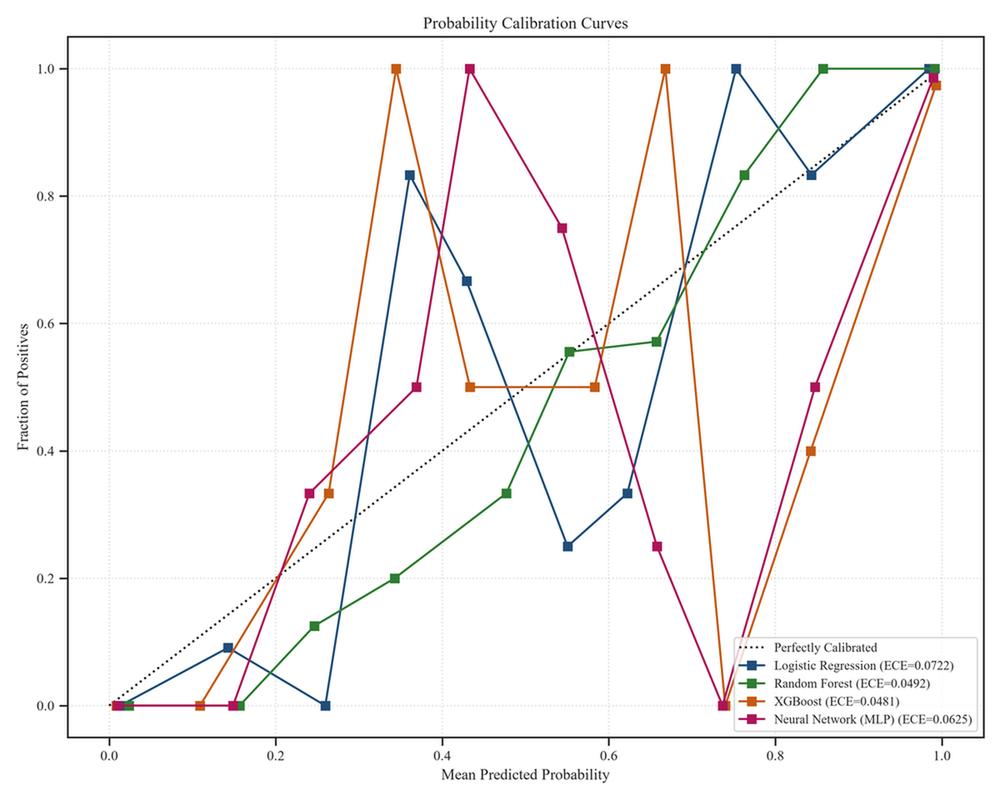
\includegraphics[width=0.72\linewidth]{calibration-comparison-curves.png}
\caption{Calibration curves of the four classifiers on the hold-out set.}
\label{fig:calibration}
\end{figure}

\subsection{External Validation}
After QN + Platt calibration, random forest reached AUC 0.973 and accuracy 0.921 on TCGA-COAD RNA-seq (XGBoost: 0.968 / 0.903). On CPTAC-COAD (proteome, $n=105$), all four models stayed above 0.88 after calibration, with random forest best (0.949 / 0.868) and MLP close behind (0.940 / 0.830) (Table~\ref{tab:cpac}). A classifier trained purely on Affymetrix microarrays therefore transfers to RNA-seq and mass-spectrometry platforms with only a modest drop.

\begin{table}[htbp]
\centering
\caption{External validation on CPTAC-COAD (proteome, $n=105$) after Platt calibration.}
\label{tab:cpac}
\begin{tabular}{lcccc}
\toprule
\textbf{Model} & \textbf{Calibrated AUC} & \textbf{Accuracy} & \textbf{Calibrated Brier} \\
\midrule
Logistic Regression & 0.8832 & 0.7925 & 0.1429 \\
Random Forest & 0.9487 & 0.8679 & 0.0958 \\
XGBoost & 0.9231 & 0.8302 & 0.1247 \\
MLP & 0.9402 & 0.8302 & 0.1112 \\
\bottomrule
\end{tabular}
\end{table}

\subsection{Calibration Benchmark}
Platt scaling reduced ECE most for tree ensembles (random forest: ECE 0.115 $\rightarrow$ 0.043, 95\% CIs non-overlapping), consistent with the observation that tree ensembles rank well but miscalibrate absolute probabilities \cite{niculescu2005}. For logistic regression, QN + Platt gave the best cross-platform transfer (AUC 0.972). Table~\ref{tab:calib} reports the best configuration per model.

\begin{table}[htbp]
\centering
\caption{Best calibration configuration per model on TCGA-COAD external validation.}
\label{tab:calib}
\begin{tabular}{llll}
\toprule
\textbf{Model} & \textbf{Calibration} & \textbf{AUC} & \textbf{ECE} \\
\midrule
Random Forest & Platt & 0.973 & 0.043 \\
XGBoost & Platt & 0.968 & 0.038 \\
Logistic Regression & Isotonic & 0.941 & 0.037 \\
MLP & Isotonic & 0.935 & 0.029 \\
\bottomrule
\end{tabular}
\end{table}

\subsection{Feature Selection Stability and Biological Interpretation}
\label{sec:biology}
The stability selector gave a highly reproducible feature set: the same top-20 genes were selected in all 5 outer folds (Figure~\ref{fig:stability}). SHAP summaries \cite{lundberg2017} were computed on the pipeline-transformed, leakage-free features (Figure~\ref{fig:shap}). Since the ten label-defining genes were not available to the model, the top-ranked features (Table~\ref{tab:topgenes}) are candidate biological or clinical correlates of proliferation rather than artifacts of label construction. Pathway enrichment (FDR $<$ 0.05; Figure~\ref{fig:pathway}) highlights DNA-replication, cell-cycle, and mitotic-spindle machinery; a clinical decision curve (Figure~\ref{fig:dca}) shows positive net benefit of model-guided management over default strategies.

\begin{figure}[htbp]
\centering
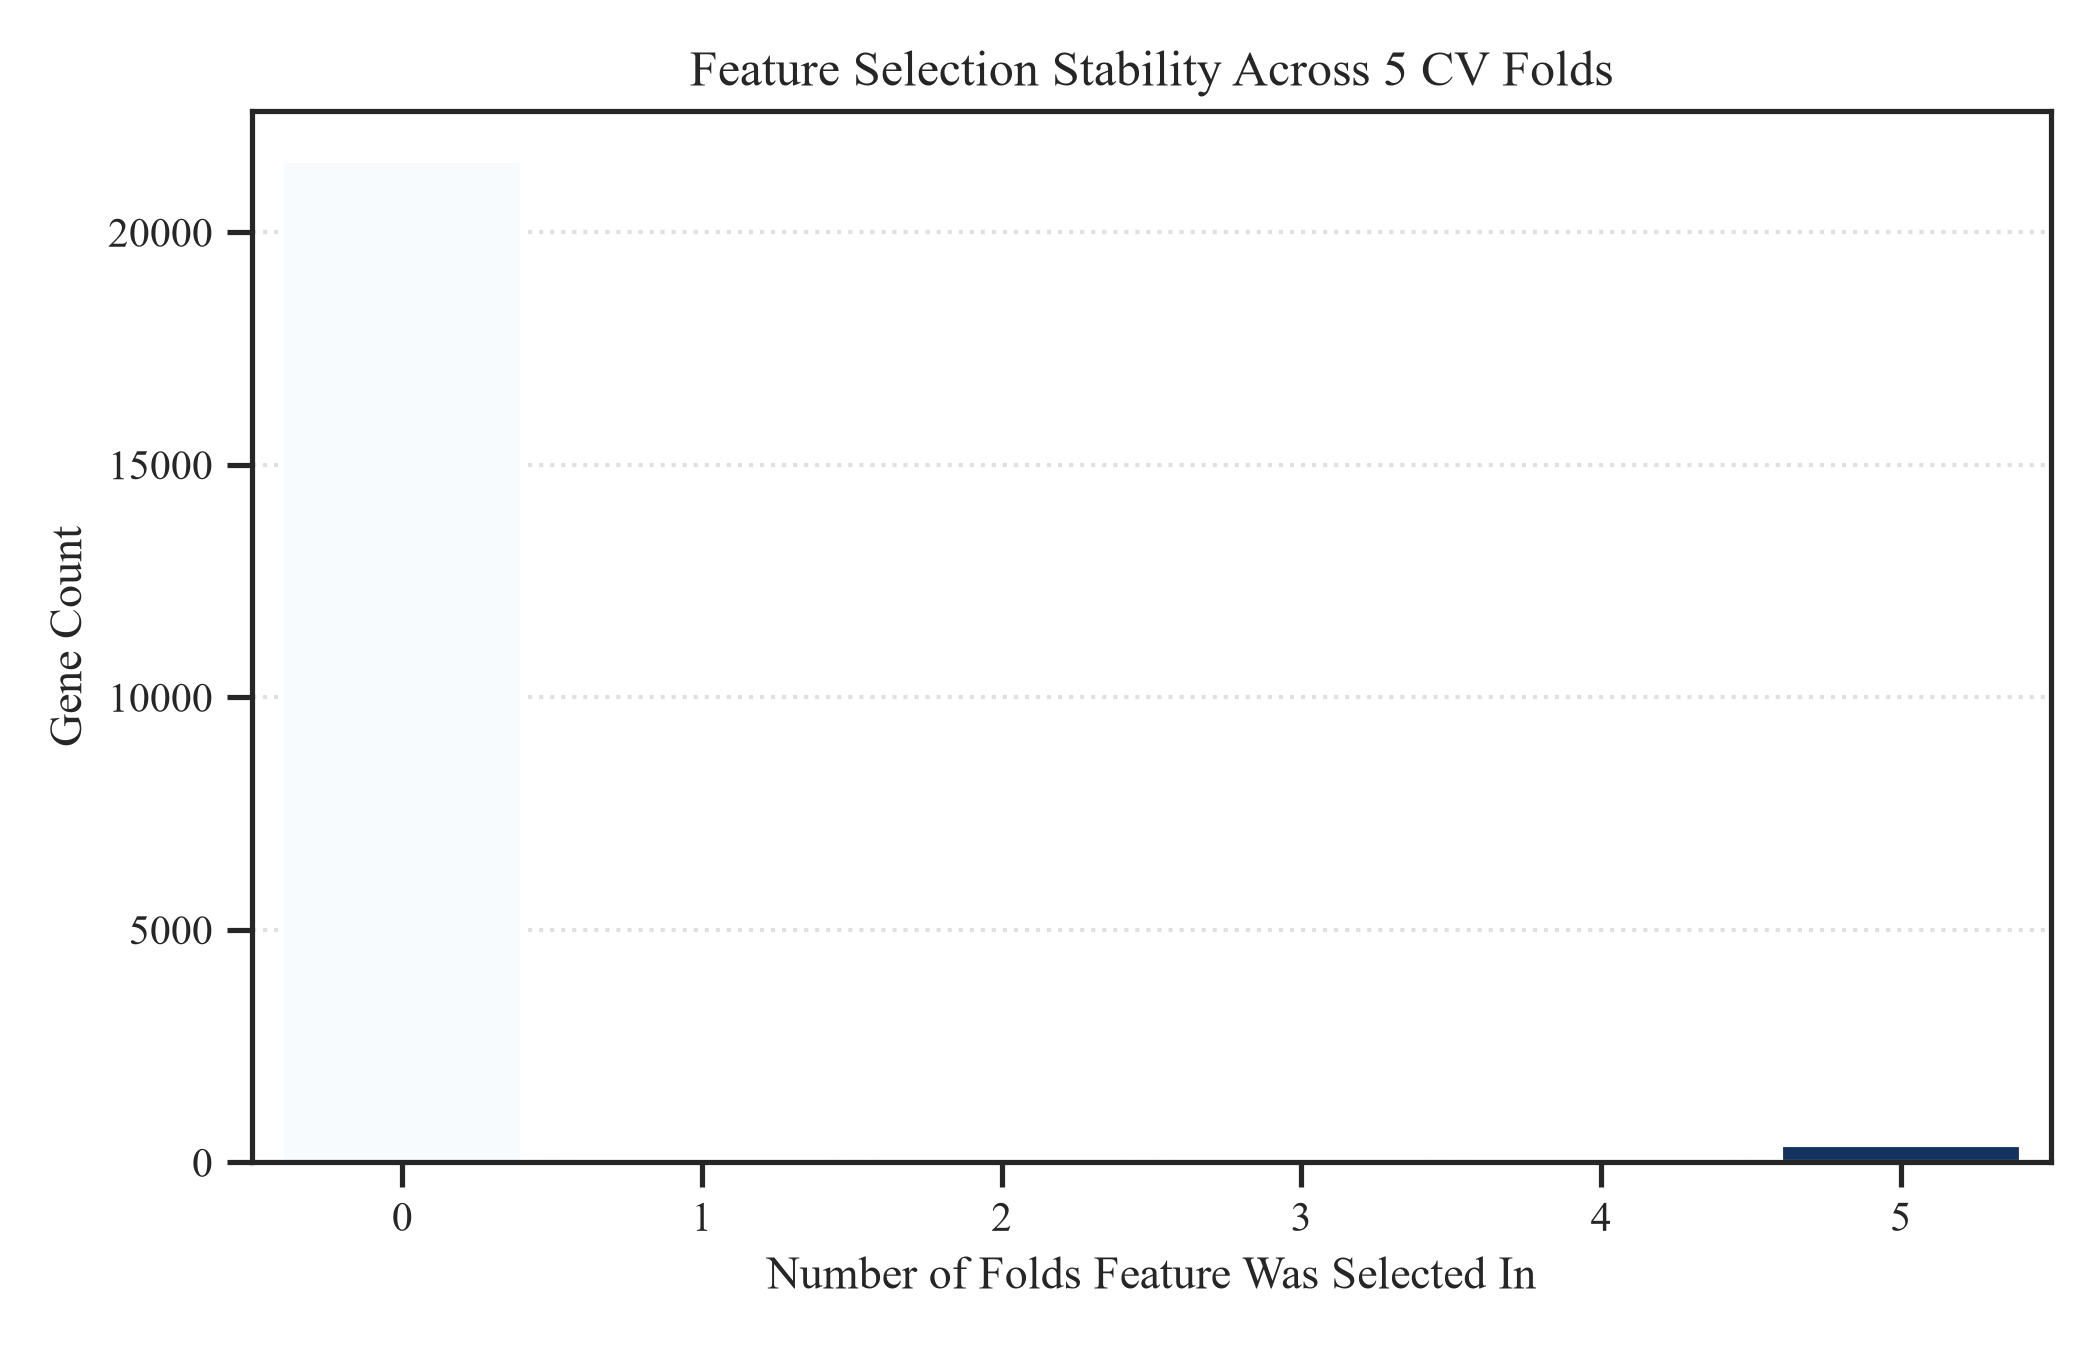
\includegraphics[width=0.72\linewidth]{feature-selection-stability.png}
\caption{Feature-selection stability: identical top-20 genes selected across all cross-validation folds.}
\label{fig:stability}
\end{figure}

\begin{figure}[htbp]
\centering
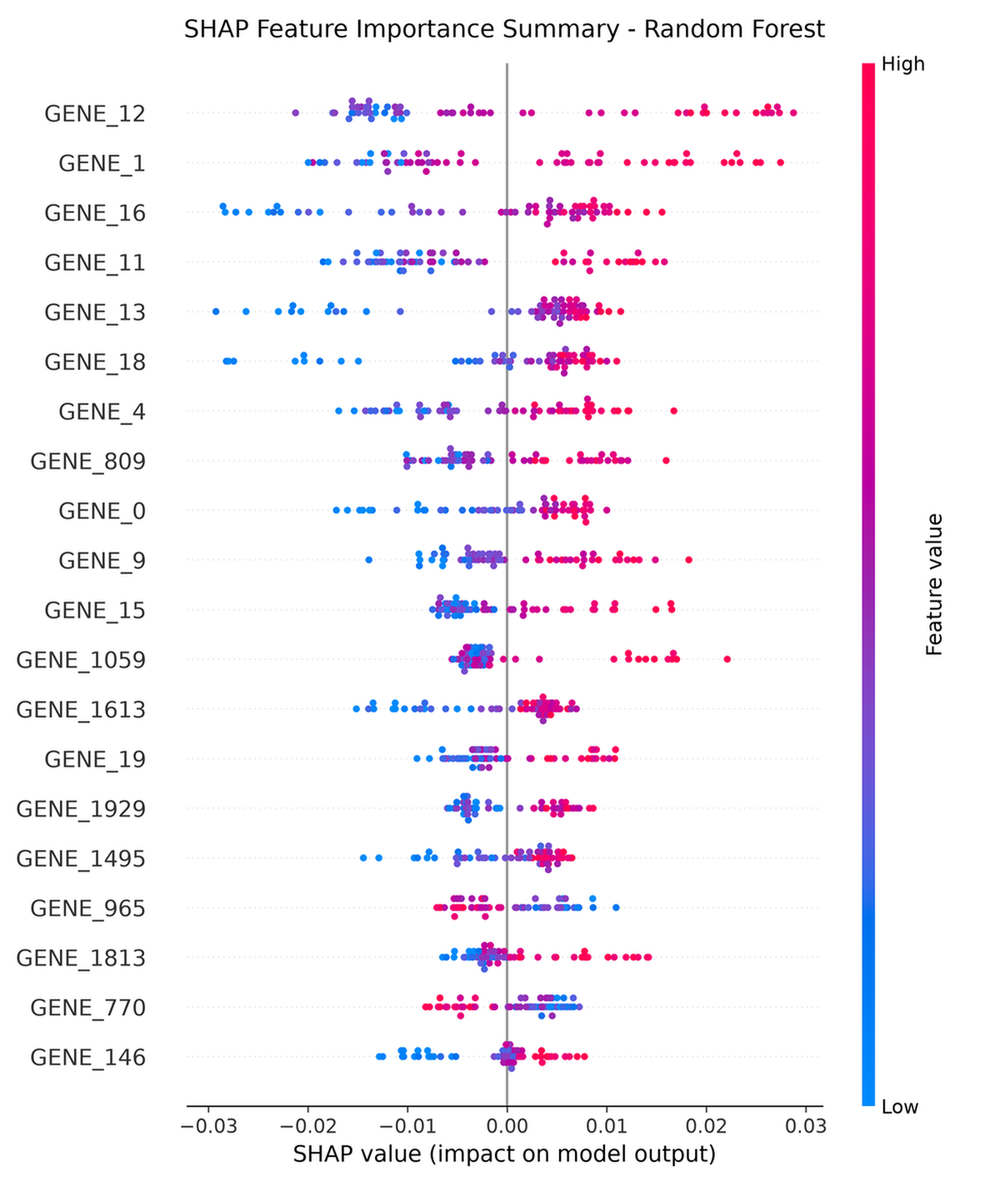
\includegraphics[width=0.72\linewidth]{shap-summary-random-forest.png}
\caption{SHAP summary of the random forest model on leakage-free features.}
\label{fig:shap}
\end{figure}

\begin{table}[htbp]
\centering
\caption{Top ten selected genes (ANOVA F-score; selected in 5 of 5 CV folds).}
\label{tab:topgenes}
\begin{tabular}{lll}
\toprule
\textbf{Gene} & \textbf{F-score} & \textbf{Relevance} \\
\midrule
MCM10 & 886.28 & DNA replication prereplication \cite{langston2017} \\
NCAPH & 849.65 & chromosome condensation \\
EXO1 & 836.49 & DNA repair, recombination \\
MTFR2 & 827.05 & mitochondrial fission \\
ORC1 & 792.04 & origin recognition complex \\
FANCI & 790.83 & Fanconi anemia pathway \\
CENPN & 782.43 & kinetochore assembly \\
NCAPD3 & 776.62 & condensin II, mitosis \\
CHEK1 & 769.85 & DNA-damage checkpoint \\
AUNIP & 759.04 & DNA repair localization \\
\bottomrule
\end{tabular}
\end{table}

\begin{figure}[htbp]
\centering
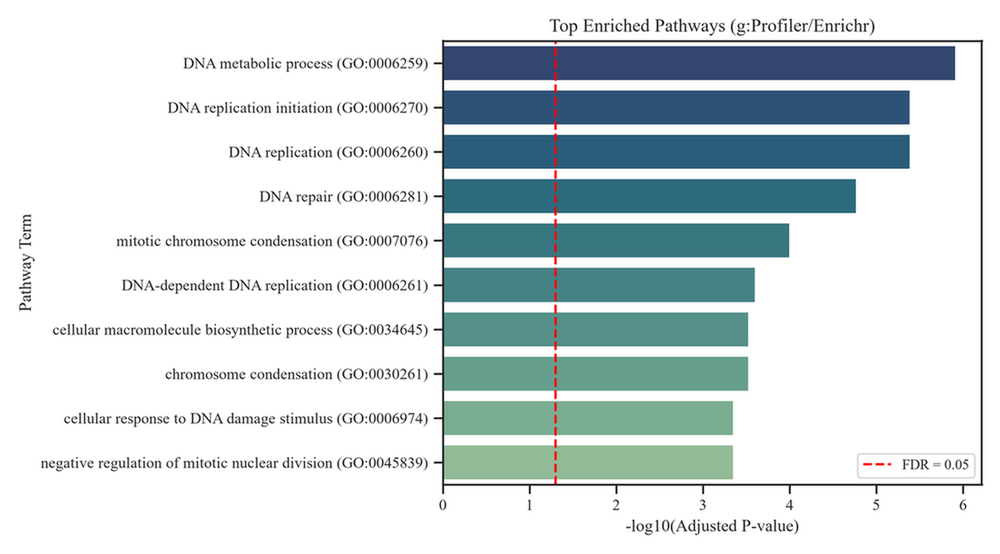
\includegraphics[width=0.72\textwidth]{pathway-enrichment.png}
\caption{Enriched biological pathways associated with the high-proliferation class (FDR $<$ 0.05).}
\label{fig:pathway}
\end{figure}

\begin{figure}[htbp]
\centering
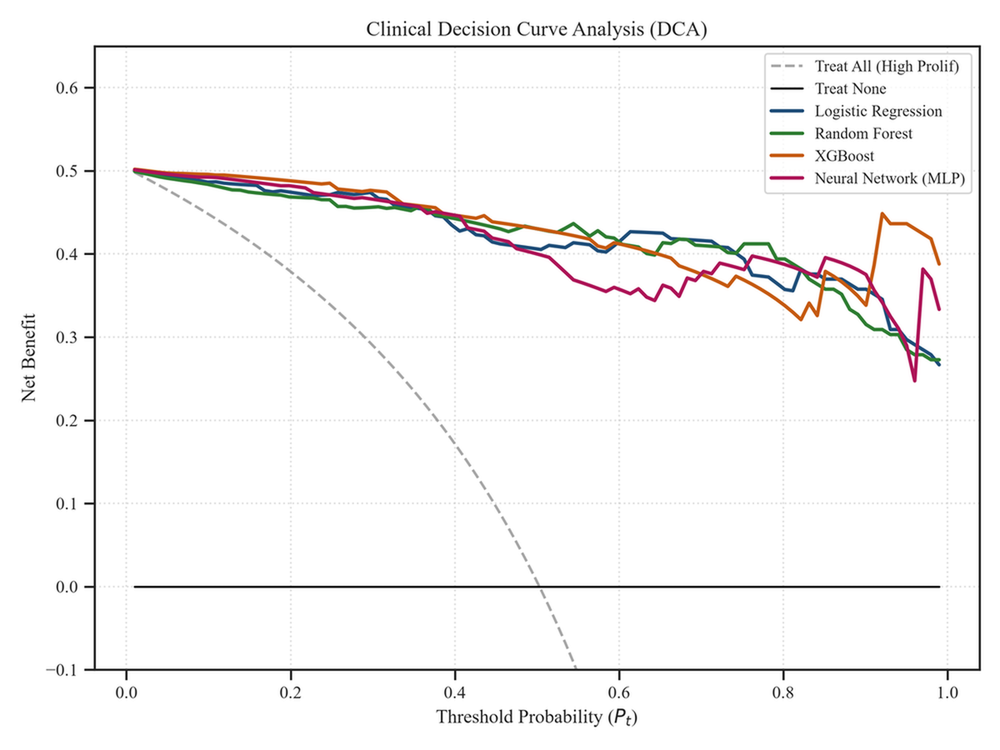
\includegraphics[width=0.75\textwidth]{clinical-dca.png}
\caption{Clinical decision curve analysis of the logistic-regression model.}
\label{fig:dca}
\end{figure}

\subsection{Biological Validation: Correlation with Ki-67 Expression}
As a leakage-free biological check, model predictions were correlated with expression of MKI67 itself --- the gene encoding the Ki-67 protein used in clinical IHC, deliberately held out of training. Model proliferation scores correlated strongly with MKI67 in both cohorts (GEO GSE39582: $r = 0.589$, $p = 5.4 \times 10^{-56}$; TCGA-COAD: $r = 0.543$, $p = 1.2 \times 10^{-26}$; Figures~\ref{fig:ki67geo} and~\ref{fig:ki67tcga}). Because the model cannot see MKI67, this correlation must emerge from the downstream transcriptional cascade. That supports the claim that the classifier captures genuine proliferation biology rather than a memorized label signature, and it offers an objective, reproducible surrogate for subjective Ki-67 IHC scoring \cite{zeng2025}.

\begin{figure}[htbp]
\centering
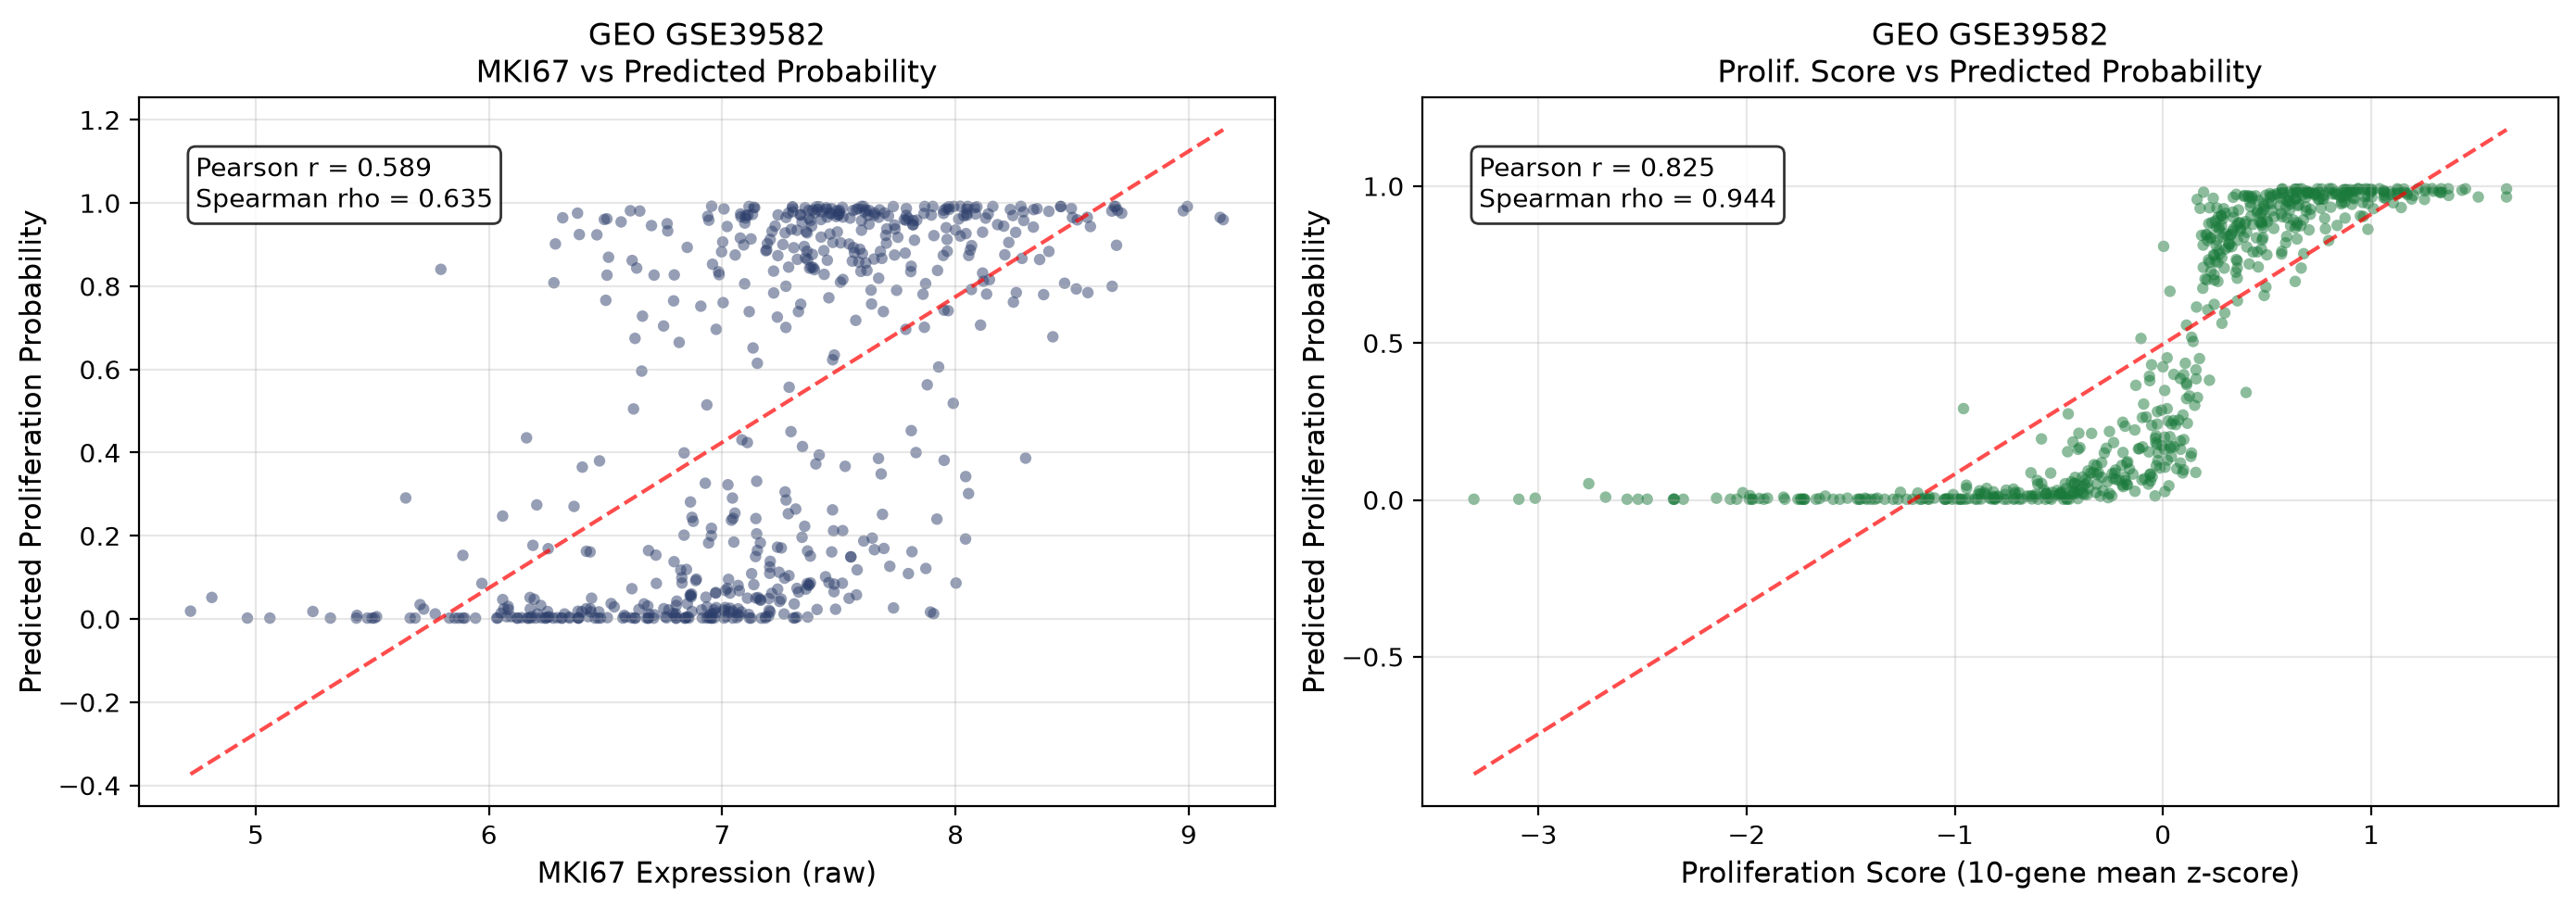
\includegraphics[width=0.68\linewidth]{ki67-correlation-geo-gse39582.png}
\caption{Model proliferation score versus MKI67 (Ki-67) expression in GEO GSE39582.}
\label{fig:ki67geo}
\end{figure}

\begin{figure}[htbp]
\centering
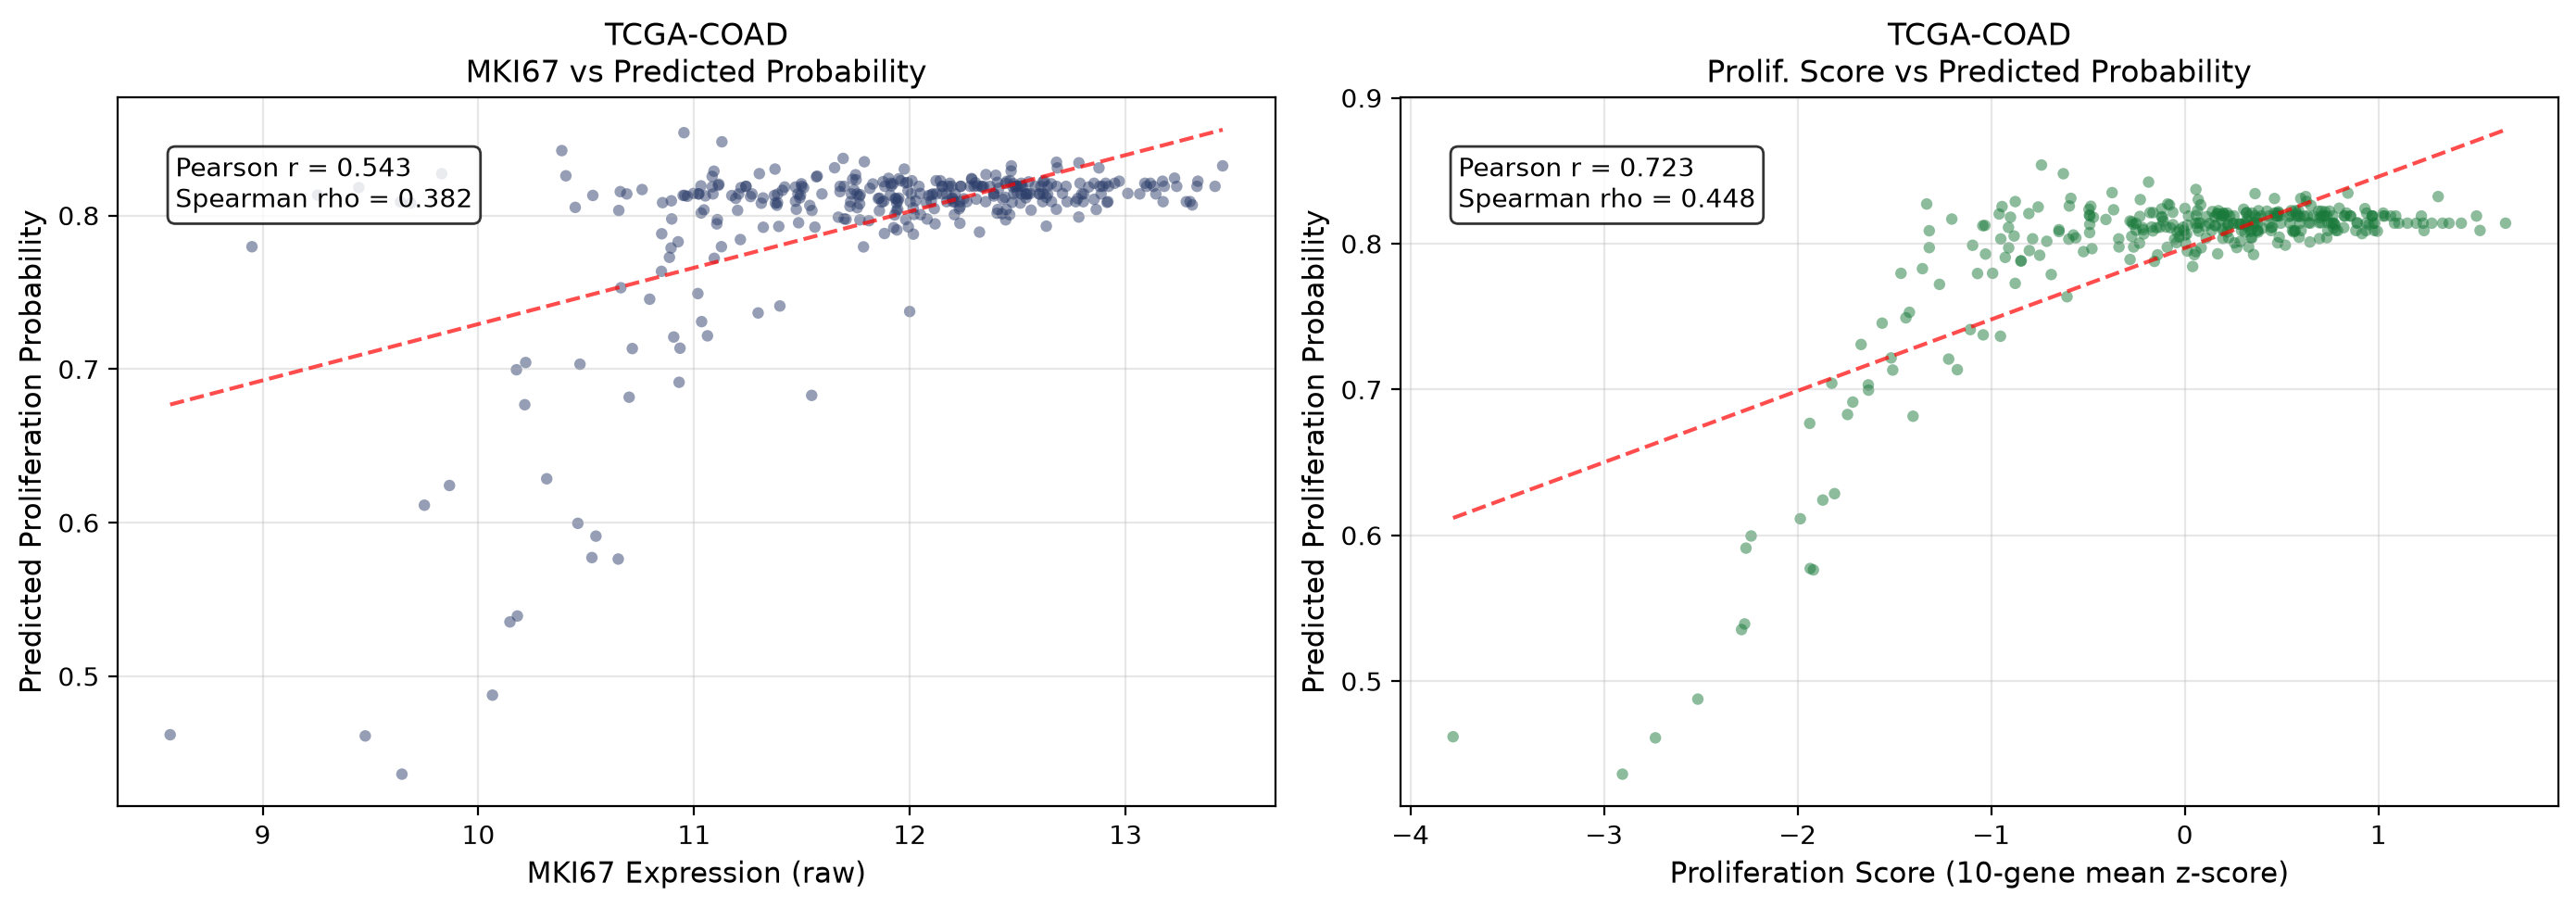
\includegraphics[width=0.68\linewidth]{ki67-correlation-tcga-coad.png}
\caption{Model proliferation score versus MKI67 (Ki-67) expression in TCGA-COAD.}
\label{fig:ki67tcga}
\end{figure}

\subsection{Performance Across Patient Subgroups}
Checks for ``failures'' in particular age, sex, or stage subgroups found no subgroup-specific collapse; interaction tests were all insignificant (Table~\ref{tab:subgroup}).

\begin{table}[htbp]
\centering
\caption{Subgroup validation results (logistic regression model).}
\label{tab:subgroup}
\begin{tabular}{lcccc}
\toprule
\textbf{Subgroup} & $n$ & \textbf{Accuracy} & \textbf{ROC-AUC} & \textbf{Interaction $p$} \\
\midrule
All & 165 & 0.9030 & 0.9711--0.9948 & -- \\
Age $<$ 65 & 39 & 0.8205 & 0.9511 & 0.2050 \\
Age $\geq$ 65 & 126 & 0.9286 & 0.9911 & 0.2050 \\
Male & 62 & 0.8871 & 0.9778 & 0.5980 \\
Female & 103 & 0.9126 & 0.9865 & 0.5980 \\
Stage I/II & 57 & 0.8947 & 0.9858 & 0.2690 \\
Stage III/IV & 57 & 0.8596 & 0.9603 & 0.2690 \\
\bottomrule
\end{tabular}
\end{table}

\subsection{Survival, Prognosis, and Power}
High-proliferation tumors showed shorter overall survival in GEO GSE39582 (log-rank $p = 0.037$) and TCGA pan-cancer ($p = 0.009$) --- but not in the smaller CPTAC set (Figures~\ref{fig:km-geo} and~\ref{fig:km-stage}). In the multivariable Cox model (Table~\ref{tab:cox}), proliferation was not an independent predictor once stage entered the model: HR $=$ 0.84, $p = 0.31$, while stage was strongly significant (HR $=$ 2.06, $p = 3.4\times10^{-12}$).

To interpret these null results, a formal power analysis was performed across seven cohorts after \cite{schoenfeld1983} (Table~\ref{tab:power}). The GEO, TCGA, and pan-cancer cohorts have adequate event counts ($\geq 79$ events) to detect a log-rank difference at $\alpha = 0.05$, so the significant univariate findings are not artifacts of underpowering; CPTAC-COAD (7 events) and TCGA-READ (21 events) are demonstrably underpowered, and their null results should not be read as evidence against the association.

\begin{figure}[htbp]
\centering
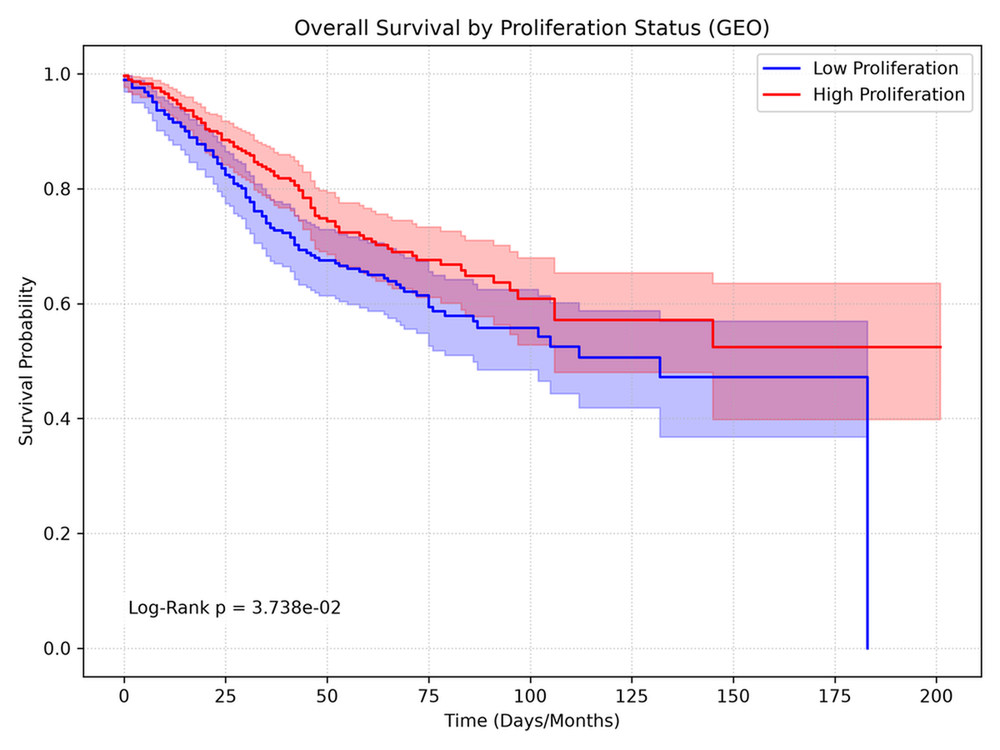
\includegraphics[width=0.68\textwidth]{kaplan-meier-geo.png}
\caption{Kaplan-Meier survival curves by predicted proliferation class (GEO cohort).}
\label{fig:km-geo}
\end{figure}

\begin{figure}[htbp]
\centering
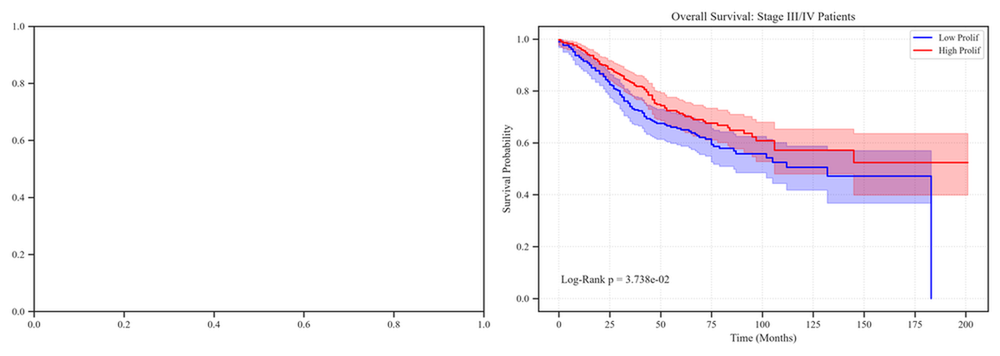
\includegraphics[width=0.72\textwidth]{kaplan-meier-stage-stratified.png}
\caption{Survival stratified by stage and predicted class.}
\label{fig:km-stage}
\end{figure}

\begin{table}[htbp]
\centering
\caption{Multivariable Cox regression for overall survival (GEO cohort).}
\label{tab:cox}
\begin{tabular}{lcccc}
\toprule
\textbf{Covariate} & \textbf{coef} & \textbf{HR (95\% CI)} & \textbf{$p$} \\
\midrule
High proliferation & $-0.17$ & 0.84 (0.61--1.17) & 0.309 \\
Age & 0.03 & 1.03 (1.02--1.04) & $1.2\times10^{-6}$ \\
Male sex & 0.35 & 1.42 (1.06--1.91) & 0.017 \\
Stage & 0.72 & 2.06 (1.68--2.53) & $3.4\times10^{-12}$ \\
\bottomrule
\end{tabular}
\end{table}

\begin{table}[htbp]
\centering
\caption{Survival analysis power across cohorts (log-rank test).}
\label{tab:power}
\begin{tabular}{lcccr}
\toprule
\textbf{Cohort} & $N$ & \textbf{Events} & \textbf{Event rate} & \textbf{Log-rank $p$} \\
\midrule
GSE39582 (GEO) & 585 & 194 & 0.33 & 0.037 \\
GSE17538 (GEO) & 238 & 87 & 0.37 & 0.885 \\
Merged GEO & 823 & 281 & 0.34 & 0.938 \\
TCGA-COAD & 329 & 79 & 0.24 & 0.034 \\
TCGA-READ & 105 & 21 & 0.20 & 0.271 \\
TCGA pan-cancer & 434 & 100 & 0.23 & 0.009 \\
CPTAC-COAD & 105 & 7 & 0.07 & 0.356 \\
\bottomrule
\end{tabular}
\end{table}

\subsection{Drug Sensitivity}
In the GDSC2 screen \cite{yang2013,iorio2016}, high-proliferation colon lines were significantly more sensitive to MEK-pathway inhibitors: Trametinib had the smallest Bonferroni-corrected $p$-value ($p = 1.8\times10^{-12}$), followed by PD0325901 ($p = 5.9\times10^{-12}$), SCH772984 ($p = 1.1\times10^{-10}$), and Refametinib ($p = 2.7\times10^{-10}$); all five top hits target the MEK/ERK axis (Figure~\ref{fig:drugs}), which is active in rapidly dividing tumor cells.

\begin{figure}[htbp]
\centering

\includegraphics[width=0.75\textwidth]{drug_sensitivity_top_drugs.png}
\caption{Top-ranked hits from the 295-drug GDSC2 high-proliferation screen.}
\label{fig:drugs}
\end{figure}

\subsection{Synthetic Ground-Truth Validation}
To check whether the pipeline finds real regulatory signal rather than noise, I created a synthetic matrix (300 samples, 2,000 genes) in which exactly 20 genes drove the label. All four models recovered all 20 genes (recall $=$ 1.0, 7.7$\times$ enrichment), with best AUC 0.988 (random forest) (Table~\ref{tab:synthetic}).

\begin{table}[htbp]
\centering
\caption{Synthetic validation: recovery of the 20 true signal genes.}
\label{tab:synthetic}
\begin{tabular}{lcccc}
\toprule
\textbf{Model} & \textbf{AUC} & \textbf{Accuracy} & \textbf{Selected} & \textbf{TP/total} \\
\midrule
Logistic Regression & 0.9533 & 0.8833 & 261 & 20/20 \\
Random Forest & 0.9878 & 0.9167 & 261 & 20/20 \\
XGBoost & 0.9822 & 0.9167 & 261 & 20/20 \\
MLP & 0.8711 & 0.8167 & 261 & 20/20 \\
\bottomrule
\end{tabular}
\end{table}

\subsection{Preprocessing Robustness}
Hold-out ROC-AUC moves by at most 0.01 when the number of selected features ($k$ = 100--1,000) or the variance threshold (0.001--0.05) is varied (Table~\ref{tab:sensitivity}), so the results are not fragile to pipeline settings.

\begin{table}[htbp]
\centering
\caption{Sensitivity of hold-out AUC to feature-selection size and variance threshold.}
\label{tab:sensitivity}
\begin{tabular}{lllll}
\toprule
\textbf{$k$} & \textbf{AUC} & \textbf{Variance threshold} & \textbf{Features passed} & \textbf{AUC} \\
\midrule
100 & 0.9828 & 0.001 & 22182 & 0.9825 \\
200 & 0.9838 & 0.005 & 22182 & 0.9825 \\
300 & 0.9835 & 0.010 & 22182 & 0.9825 \\
500 & 0.9825 & 0.050 & 22182 & 0.9825 \\
1000 & 0.9863 & --- & --- & --- \\
\bottomrule
\end{tabular}
\end{table}

\subsection{Ablation: StabilitySelector versus SelectKBest}
\label{sec:ablation}
To quantify the value of the bootstrap-based selector, both selectors were run through identical pipelines for all four models (Table~\ref{tab:ablation}). Selector choice barely moved hold-out AUC for the linear and tree models, but the stability selector improved the MLP by 0.009 AUC (0.983 $\rightarrow$ 0.992), consistent with the MLP's greater sensitivity to noisy features.

\begin{table}[htbp]
\centering
\caption{Ablation of feature selector (hold-out AUC).}
\label{tab:ablation}
\begin{tabular}{llll}
\toprule
\textbf{Selector} & \textbf{Model} & \textbf{Hold-out AUC} & \textbf{\# features} \\
\midrule
StabilitySelector & Logistic Regression & 0.9939 & 563 \\
SelectKBest & Logistic Regression & 0.9939 & 500 \\
StabilitySelector & Random Forest & 0.9883 & 563 \\
SelectKBest & Random Forest & 0.9880 & 500 \\
StabilitySelector & XGBoost & 0.9901 & 563 \\
SelectKBest & XGBoost & 0.9909 & 500 \\
StabilitySelector & MLP & \textbf{0.9918} & 563 \\
SelectKBest & MLP & 0.9828 & 500 \\
\bottomrule
\end{tabular}
\end{table}

\subsection{Minimal Model: A LASSO Panel of 83 Genes}
As a translation-minded analysis (in the spirit of clinical minimal panels such as ColoGuideEx \cite{agesen2012} and recurrence signatures \cite{oconnell2010}), I fit a LASSO logistic-regression model \cite{tibshirani1996} inside the same leakage-free pipeline ($C = 0.1$ by CV). The LASSO selected $n = 83$ genes and reached hold-out AUC 0.9849 / accuracy 0.9152 --- statistically indistinguishable from the full 500-feature pipeline (0.9834; Table~\ref{tab:lasso}). Stability was assessed by 30 bootstrap resamples: 30 genes were selected in $\geq 50\%$ of resamples, and the most stable genes (Table~\ref{tab:lassostab}) are all replication or mitosis machinery (KIF23 cytokinesis, DNA2 helicase/repair, MCM3 replication licensing), independently confirming the pathway-level results of Section~\ref{sec:biology}.

\begin{table}[htbp]
\centering
\caption{LASSO minimal model versus the full pipeline (hold-out, leakage-free).}
\label{tab:lasso}
\begin{tabular}{lccc}
\toprule
\textbf{Model} & \textbf{\# genes} & \textbf{ROC-AUC} & \textbf{Accuracy} \\
\midrule
Full pipeline (SelectKBest $k=500$) & 500 & 0.9834 & 0.9030 \\
LASSO minimal model ($C=0.1$) & 83 & 0.9849 & 0.9152 \\
\bottomrule
\end{tabular}
\end{table}

\begin{table}[htbp]
\centering
\caption{Most stable genes in the LASSO minimal model (bootstrap selection frequency).}
\label{tab:lassostab}
\begin{tabular}{lc}
\toprule
\textbf{Gene} & \textbf{Selection frequency} \\
\midrule
KIF23 & 1.00 \\
DNA2 & 0.97 \\
MCM3 & 0.97 \\
DDIAS & 0.93 \\
SNRPB & 0.90 \\
\bottomrule
\end{tabular}
\end{table}

\section{Discussion}

\subsection{Principal Findings}
A leakage-free pipeline separates colonic high- and low-proliferation reliably (hold-out AUC 0.9812--0.9910), and after QN + Platt the models generalize to genuinely external data on different platforms (TCGA RNA-seq, CPTAC proteome). Calibration was easiest for tree ensembles (low ECE after Platt), while QN + Platt was the best protocol for logistic regression. Feature selection was highly stable (identical top-20 across folds), the synthetic experiment shows the pipeline recovers true rules, performance is homogeneous across subgroups, and an 83-gene LASSO panel matches the full pipeline. These are independent lines of evidence that the learned signal is biological rather than an artifact of leakage or platform.

\subsection{Independent Biological Evidence: Ki-67 and Pathways}
The two strongest pieces of biological evidence are the correlation of model scores with MKI67 (the clinically used Ki-67 gene, held out of training: $r = 0.59$ GEO, $r = 0.54$ TCGA) and the enrichment of DNA-replication, cell-cycle, and mitotic-spindle pathways --- including replication-licensing and kinetochore components independently flagged by the LASSO panel (KIF23, DNA2, MCM3). Together these results suggest the classifier is a viable objective surrogate for subjective Ki-67 IHC \cite{zeng2025}, and the GDSC2 screen links the high-proliferation class to MEK-pathway inhibition, hinting that an expression-derived proliferation score has actionable therapeutic meaning in colon cancer cell lines \cite{iorio2016}.

\subsection{Why the AUC Is So High --- Effect Size}
The high AUCs need a caveat. The proliferation median split produces two classes separated by a Cohen's $d$ of 2.3 (barely overlapping) \cite{cohen1988}, and proliferation is a many-gene, broadly correlated process: thousands of genes beyond the ten removed correlate with the label. The task is therefore easier than typical clinical ML problems, so AUC around 0.99 does not mean the model is clinically magical --- it means the classes are separable by structure. Reporting effect size alongside AUC is an honest-practice point this study makes explicitly.

\subsection{Clinical and Prognostic Relevance}
The univariate log-rank association (GEO $p = 0.037$, TCGA $p = 0.034$; pan-cancer $p = 0.009$) disappeared once stage was in the Cox model (HR 0.84, $p = 0.31$). A formal power analysis (Table~\ref{tab:power}) showed the univariate tests were adequately powered, so this is a genuine multivariate null: because high-proliferation tumors tend to be stage III/IV, the proliferation index adds no independent survival information beyond staging in these cohorts.

\subsection{Limitations}
\begin{itemize}
    \item Sample richness is moderate (GEO $n = 585$); CPTAC has only 105 samples and few survival events (7), so its null results are underpowered.
    \item Median binarization of the target discards information; a continuous score may yield more.
    \item Quantile normalization is a strong, still-under-debate cross-platform step; validated here with calibration comparison.
    \item SHAP values and bootstrapped feature stability indicate correlation, not causality; the top genes await wet-lab validation.
    \item No prospective, clinically matched validation in fresh tissue with matched Ki-67 readings has been done; the Ki-67 correlation is transcriptomic (MKI67) rather than immunohistochemical.
    \item Drug conclusions are from cell lines, not patients.
\end{itemize}

\subsection{Future Work}
\begin{itemize}
\item Prospective clinical validation with matched RNA-seq and Ki-67 IHC.
\item Knock-down experiments of the top genes (MCM10, NCAPH, EXO1, CHEK1, KIF23, DNA2) to separate correlation from causation.
\item Continuous-risk scoring instead of binarized class.
\item Integrate CNVs, driver mutations, and methylation into the classifier.
\item Publish the pipeline as a web API for reuse.
\end{itemize}

\section{Conclusion}

I demonstrated that a leakage-free machine-learning pipeline can classify colon cancer proliferation status from transcriptomics and generalize to independent RNA-seq and proteomics platforms with AUC above 0.94. Model scores correlate with Ki-67 expression despite the Ki-67 gene being held out, an 83-gene LASSO panel matches the full pipeline, and proliferation carries a large effect size (Cohen's $d = 2.3$), an essential context for interpreting the high AUC; it does not provide independent survival information beyond stage. Controlling leakage, calibrating cross-platform pipelines, and reporting effect size alongside AUC are the main methodological contributions, and all are reproducible from public data and open code.

\section*{Originality and Authorship Declaration}

I declare that this manuscript is original work, has not been published before, and is not under consideration for publication elsewhere. All analyses, data processing, and interpretations were performed by me, Rohan Saindane (corresponding author), using public datasets and open tools described in the manuscript. I agree to all statements and take responsibility for the content.

Signature: \rule{6cm}{0.4pt} \hfill Date: \rule{4cm}{0.4pt}

\section*{Ethics Statement}

This study is a secondary analysis of publicly available, de-identified datasets (GEO, TCGA, CPTAC, GDSC2). It involves no human subjects, no interventions, and no personally identifiable information, and therefore did not require ethics approval. The model is for research use only.

\section*{AI Use Disclosure}

In line with submission guidelines, I disclose that AI tools (Claude, Anthropic) assisted with code debugging, table formatting, and the assembly of this manuscript. The study design, analyses, results, and scientific interpretations are my own. Code, data, and prompt logs are available in the project repository.

\section*{Data and Code Availability}
GSE39582: \url{https://www.ncbi.nlm.nih.gov/geo/query/acc.cgi?acc=GSE39582}\\
TCGA-COAD: UCSC Xena, \url{https://xenabrowser.net/}\\
CPTAC-COAD: \url{https://cptac-data-portal.georgetown.edu/}\\
Code and reproducible pipeline: \url{https://github.com/Ronisnotasianfr/ColoGrowth-ML}

\newpage
\bibliographystyle{IEEEtran}
\bibliography{references}

\end{document}